\def\cG{\mathcal{G}}
\def\rr{\mathbb{R}}

\section{Accelerating GaLore with Second-Order Information}
Generative LLMs are trained with respect to the Causal Language Model (CLM) objective, where the task is to predict the next token in a sequence based solely on the tokens that have come before it. This approach is called ``causal'' because it respects the temporal order of language, ensuring that the model's predictions at any point depend only on past and not future inputs.

Given a sequence of tokens \( x = (x_1, x_2, \dots, x_T) \), the causal language model aims to maximize the likelihood of the sequence by decomposing it into a product of conditional probabilities:

\[
\text{Prob}_{\theta}(x) = \prod_{t=1}^T \text{Prob}_{\theta}(x_t \mid x_{<t})
\]

where:

\begin{itemize}
    \item \( x_{<t} = (x_1, x_2, \dots, x_{t-1}) \) represents all tokens before position \( t \).
    \item \( \text{Prob}_{\theta}(x_t \mid x_{<t}) \) is the probability of the next token given all previous tokens and \( \theta \in \Theta \) where \( \Theta\) is the space of all model parameters.
\end{itemize}

The training objective is to minimize the \textit{negative log-likelihood (NLL)} of the observed sequences, which is equivalent to minimizing the \textit{cross-entropy loss} between the predicted probability distribution and the actual next token:

\[
\Phi(\theta) = -\sum_{t=1}^T \log \text{Prob}_{\theta}(x_t \mid x_{<t})
\]

This loss penalizes the model more when it assigns lower probabilities to the correct next token. By minimizing this loss, the model learns to assign higher probabilities to appropriate continuations of text.

Now gradient descent algorithms are iterative in nature, where the goal at each step is to find the optimal update direction $\mathbf{\delta}$ that locally minimizes the loss function. Now in the case of GaLore, the update direction can be parameterized as: \(\mathbf{\delta} = \mathbf{P^T u}\), where \(\mathbf{P} \in \mathbb{R}^{r\text{x}n}\) is the projection matrix, which means that the Taylor series expansion for that update is given by:

\[
\Phi(\theta - \mathbf{P^T u}) \approx \Phi(\theta) - \mathbf{g^T P^T u} + \frac{1}{2} \mathbf{u^T PHP^T  u}
\]

where \(\mathbf{g} = \nabla_{\theta} \Phi(\theta)\) is the gradient and \(\mathbf{H} = \nabla^2_{\theta} \Phi(\theta)\) is the Hessian Matrix. Then the problem of finding the optimal direction in the low rank space is given by:

\[
\mathbf{u^*} = \argmin_{u\in \mathbb{R}^r} \{\Phi(\theta_{k}) - \mathbf{g^T P^T u} + \frac{1}{2} \mathbf{u^T PHP^T  u}\}
\]

which corresponds to the gradient descent update given by:

\[
\theta_{k+1} = \theta_{k} - \alpha_{k} \mathbf{P^T u^*}
\]

for some learning rate $\alpha_{k}$ at the $k^{\text{th}}$ iteration.

In GaLore, the projection matrix $\mathbf{P}$ is chosen to be the top $r$ singular vectors of the gradient matrix $\mathbf{g}$ and the solution to $u^*$ is approximated using popular optimizers like Adam, AdamW, etc. This method is memory efficient as it only requires storing the projection matrix and the costly optimizer states are now significantly reduced depending on the chosen rank $r$.





\definecolor{cus_color}{rgb}{22, 96, 55}


\makeatletter
\newcommand{\removelatexerror}{\let\@latex@error\@gobble}
\makeatother


\begin{figure}[!t]
\centering
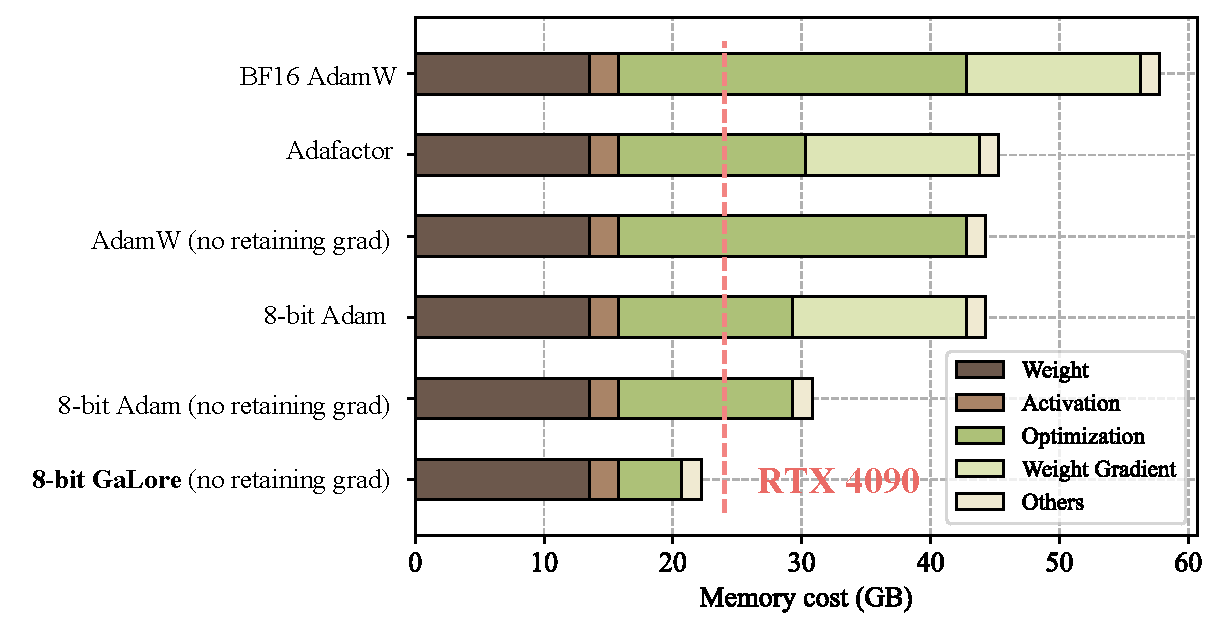
\includegraphics[width=1\columnwidth]{figures/files/memory_breakdown.pdf}
\vskip -0.11in
\caption{\small{Estimated memory consumption of pre-training a LLaMA 7B model with a token batch size of 256 on a single device, without activation checkpointing and memory offloading\protect\footnotemark[2]. Details refer to Section~\ref{sec:memory_measure}.}}
\label{fig:memory_breakdown} 
\vskip -0.15in
\end{figure}
\footnotetext[1]{The calculation is based on LLaMA architecture, BF16 numerical format, and maximum sequence length of 2048.}
\footnotetext[2]{In the figure, ``no retaining grad'' denotes the application of per-layer weight update to reduce memory consumption of storing weight gradient \citep{lvFullParameterFinetuning2023}.}
\SetAlFnt{\fontsize{8pt}{9pt}\selectfont}
\SetAlCapFnt{\fontsize{8pt}{9pt}\selectfont}
\begin{algorithm}[t]
    \SetAlgoLined
        \PyCode{for weight in model.parameters():} \\
        \Indp   %
            \PyCode{grad = weight.grad} \\ 
            \PyComment{original space -> compact space} \\
            \PyCode{lor\_grad = \textbf{project}(grad)} \\
            \PyComment{update by Adam, Adafactor, etc.} \\
            \PyCode{lor\_update = \textbf{update}(lor\_grad)} \\
            \PyComment{compact space -> original space} \\
            \PyCode{update = \textbf{project\_back}(lor\_update)} \\
            \PyCode{weight.data += update} \\
        \Indm %
    \caption{\fontsize{8pt}{9pt}\selectfont{\lowrank{}, PyTorch-like}}
    \label{alg:code_box}
\end{algorithm}


However, the performance of GaLore is still not on par with the vanilla AdamW optimizer. To bridge this gap, we propose Natural GaLore, which incorporates second-order information in the optimization process.

A property of the natural gradient is that it is \textit{Fisher efficient}, meaning that it minimizes the expected Kullback-Leibler divergence between the true and approximated distributions in a single step. 

This property is particularly useful in the context of LLMs, where the loss landscape is highly non-convex and the optimization process can be challenging.

Natural gradient methods are optimization algorithms that adjust parameter updates according to the geometry of the parameter space, leading to faster convergence compared to standard gradient descent \citep{amariNaturalGradientWorks1998}. They precondition the gradient using the inverse of the Fisher Information Matrix (FIM), effectively incorporating second-order information about the loss landscape. However, computing and storing the full FIM and its inverse is computationally infeasible for large-scale models due to their high dimensionality.

\subsection{Amari's Fisher Efficiency Result}

Natural gradient descent is known for its desirable property of being ``Fisher efficient,'' as demonstrated by \citet{amari1998natural}. This means that, under certain conditions, the estimator obtained via natural gradient descent achieves the lowest possible asymptotic variance as dictated by the Cramér-Rao lower bound. Specifically, when minimizing an objective function \( h(\theta) \) that represents the expected loss over a data distribution, natural gradient descent updates of the form
\[
\theta_{k+1} = \theta_k - \alpha_k F^{-1} g_k(\theta_k)
\]
can lead to estimators \( \theta_k \) whose variance converges to the optimal value of \( \frac{1}{k} F^{-1}(\theta^*) \) as the number of iterations \( k \) increases, where \( F(\theta^*) \) is the Fisher Information Matrix evaluated at the optimal parameter \( \theta^* \), and \( g_k(\theta_k) \) is an unbiased stochastic gradient estimate.

However, several important caveats and conditions accompany this result:

\begin{enumerate}
    \item \textbf{Assumption of Convergence to the Global Optimum}: The proof assumes that the parameter updates converge to the global optimum \( \theta^* \). While this assumption holds in convex optimization problems, it does not generally hold for non-convex objectives such as those encountered in deep neural networks. In practice, convergence to a local optimum may still allow the Fisher efficiency property to hold approximately, but this is not guaranteed.

    \item \textbf{Requirement of Exact Fisher Information Matrix Computation}: The result relies on the exact computation of the Fisher Information Matrix \( F(\theta) \) using the entire data distribution. In large-scale machine learning tasks, computing \( F(\theta) \) over the entire training set is computationally infeasible. Approximating \( F(\theta) \) using mini-batches or running estimates can introduce errors that may invalidate the Fisher efficiency guarantee.

    \item \textbf{Result Focuses on Parameter Convergence}: The Fisher efficiency result pertains to the convergence of the parameter estimates \( \theta_k \) in terms of their variance, not directly to the convergence of the objective function value \( h(\theta_k) \). While lower variance in parameter estimates is desirable, practitioners are often more interested in the optimization of the loss function. Although there is a relationship between parameter variance and loss convergence, the translation is not straightforward and may depend on additional assumptions.

    \item \textbf{Assumption of Model Realizability}: The proof assumes that the model is capable of perfectly capturing the true data distribution—referred to as ``realizability.'' This means that at the optimal parameters \( \theta^* \), the model distribution matches the data distribution exactly. In practice, models may be misspecified or have insufficient capacity, violating this assumption and potentially invalidating the Fisher efficiency result.
\end{enumerate}

Despite these caveats, natural gradient descent remains a valuable optimization method, especially when the iteration budget is limited. Here's why:

\begin{itemize}
    \item \textbf{Improved Convergence Rates in Practice}: Even if the asymptotic guarantees are compromised due to the above conditions, natural gradient descent can still offer faster convergence in the early stages of optimization. By accounting for the curvature of the loss landscape through the Fisher Information Matrix (or its approximation), natural gradient descent can take more informed steps compared to standard gradient descent, potentially escaping flat regions or navigating steep ravines more effectively.

    \item \textbf{Enhanced Performance with Limited Iterations}: In practical scenarios where computational resources or time limit the number of allowable iterations, the benefits of incorporating second-order information become more pronounced. Natural gradient descent can achieve lower loss values or better parameter estimates within a fixed iteration budget compared to first-order methods, even if the asymptotic variance reduction is not fully realized.

    \item \textbf{Reduction of the Starting Point Dependent Term}: While asymptotically the difference in performance between natural gradient descent and simpler methods may diminish, natural gradient descent can significantly reduce the constant factors associated with convergence terms that depend on the initial parameter values. This reduction can lead to practical performance gains in finite-iteration regimes.

    \item \textbf{Approximate Fisher Information Matrix Usage}: Although computing the exact Fisher Information Matrix is infeasible for large models, practical approximations or efficient estimations (such as using a limited history of gradients or employing block-diagonal or low-rank approximations) can capture enough curvature information to improve optimization without incurring prohibitive computational costs.
\end{itemize}

In conclusion, while the theoretical Fisher efficiency of natural gradient descent comes with significant assumptions that may not hold in practical settings, the method still offers substantial advantages when the number of iterations is limited. By leveraging curvature information, natural gradient descent can provide faster convergence and better optimization performance in the early stages of training large-scale models, making it a valuable tool in the machine learning practitioner's arsenal.

\begin{enumerate}
    \item \textbf{Low-Rank Gradient Projection}
    \item \textbf{Gradient History Buffer Maintenance}
    \item \textbf{FIM Approximation Using Gradient History}
    \item \textbf{Natural Gradient Computation via Woodbury Identity}
    \item \textbf{Efficient Solution Using Cholesky Decomposition}
\end{enumerate}

We explain each step in detail below.

\paragraph{Step 1: Low-Rank Gradient Projection}

\begin{algorithm}[t]
  \SetAlgoLined
  \PyCode{def \textbf{project}(full\_rank\_grad, iter):} \\
  \Indp   %
      \PyComment{Check if projection matrices need updating} \\
      \PyCode{\textbf{if} core is None \textbf{or} iter \% update\_proj\_gap == 0:} \\
      \Indp   %
          \PyCode{core, factors = get\_orthogonal\_matrix(full\_rank\_grad, rank)} \\
      \Indm   %
      \PyComment{Transform gradient to low-rank space} \\
      \PyCode{low\_rank\_grad = transform(factors, full\_rank\_grad)} \\
      \PyComment{Apply natural gradient transform} \\
      \PyCode{low\_rank\_grad = \textbf{natural\_gradient\_transform}(low\_rank\_grad)} \\
      \PyCode{\textbf{return} low\_rank\_grad} \\
  \Indm   %
  \caption{\fontsize{8pt}{9pt}\selectfont{Pseudocode for \textbf{project} method}}
  \label{alg:project_method}
\end{algorithm}


Given a full-rank gradient tensor $\mathbf{g} \in \mathbb{R}^{n_1 \times n_2 \times \cdots \times n_d}$, we project it onto a low-rank subspace using Tucker decomposition \citep{tuckerMathematicalNotesThree1966}. The Tucker decomposition approximates $\mathbf{g}$ as:

\[
\mathbf{g} \approx \mathcal{G} = \mathcal{C} \times_1 \mathbf{U}^{(1)} \times_2 \mathbf{U}^{(2)} \times_3 \cdots \times_d \mathbf{U}^{(d)},
\]

where:

\begin{itemize}
    \item $\mathcal{C} \in \mathbb{R}^{r_1 \times r_2 \times \cdots \times r_d}$ is the core tensor capturing the interaction between different modes.
    \item $\mathbf{U}^{(i)} \in \mathbb{R}^{n_i \times r_i}$ are the factor matrices (often orthogonal), representing the principal components along each mode.
    \item $\times_i$ denotes the mode-$i$ tensor-matrix product.
    \item $r_i$ is the rank along mode $i$, with $r_i \ll n_i$.
\end{itemize}

The transformed low-rank gradient is obtained by projecting $\mathbf{g}$ onto the subspace spanned by $\{\mathbf{U}^{(i)}\}$:

\[
\mathbf{g}_{\text{low}} = \text{Transform}(\mathbf{g}) = \mathbf{g} \times_1 (\mathbf{U}^{(1)})^\top \times_2 (\mathbf{U}^{(2)})^\top \times_3 \cdots \times_d (\mathbf{U}^{(d)})^\top.
\]

This results in a compact representation of the gradient in the low-rank subspace.

\paragraph{Step 2: Gradient History Buffer Maintenance}

\begin{algorithm}[t]
  \SetAlgoLined
  \PyCode{def \textbf{natural\_gradient\_transform}(low\_rank\_grad):} \\
  \Indp   %
      \PyComment{Flatten low-rank gradient to vector} \\
      \PyCode{grad\_vector = low\_rank\_grad.reshape(-1)} \\
      \PyComment{Update gradient history buffer} \\
      \PyCode{append grad\_vector to grad\_history} \\
      \PyCode{\textbf{if} len(grad\_history) > history\_size:} \\
      \Indp   %
          \PyCode{remove oldest gradient from grad\_history} \\
      \Indm   %
      \PyComment{Form matrix G from gradient history} \\
      \PyCode{G = stack(grad\_history)} \\
      \PyComment{Compute S = I + $\lambda^{-1}$ G$^\top$G} \\
      \PyCode{S = (1 / lambda\_damping) * (G$^\top$ @ G)} \\
      \PyCode{add 1.0 to diagonal elements of S} \\
      \PyComment{Compute G$^\top$ grad\_vector} \\
      \PyCode{GTg = G$^\top$ @ grad\_vector} \\
      \PyComment{Solve S z = GTg for z using Cholesky decomposition} \\
      \PyCode{L = Cholesky\_decompose(S)} \\
      \PyCode{solve L u = GTg for u} \\
      \PyCode{solve L$^\top$ z = u for z} \\
      \PyComment{Compute natural gradient} \\
      \PyCode{G\_z = G @ z} \\
      \PyCode{ng\_vector = (1 / lambda\_damping) * grad\_vector} \\
      \PyCode{ng\_vector -= (1 / lambda\_damping$^2$) * G\_z} \\
      \PyComment{Reshape back to original low-rank shape} \\
      \PyCode{natural\_grad = ng\_vector.reshape\_as(low\_rank\_grad)} \\
      \PyCode{\textbf{return} natural\_grad} \\
  \Indm   %
  \caption{\fontsize{8pt}{9pt}\selectfont{Pseudocode for \textbf{natural\_gradient\_transform}}}
  \label{alg:natural_gradient_method}
\end{algorithm}


To capture local curvature information, we maintain a buffer of recent transformed gradients. Let $\mathbf{g}_t$ be the transformed low-rank gradient at iteration $t$, flattened into a vector:

\[
\mathbf{g}_t \in \mathbb{R}^{k}, \quad \text{where } k = r_1 r_2 \cdots r_d.
\]

We store the recent $s$ gradients in the matrix $\mathbf{G}$:

\[
\mathbf{G} = [\mathbf{g}_{t - s + 1}, \mathbf{g}_{t - s + 2}, \dots, \mathbf{g}_t] \in \mathbb{R}^{k \times s}.
\]

This gradient history captures the directions of recent updates, which are informative for approximating the FIM.

\paragraph{Step 3: Approximating the Fisher Information Matrix}

We approximate the Fisher Information Matrix within the low-rank subspace using the outer products of the stored gradients:

\[
\mathbf{F} = \lambda \mathbf{I}_k + \mathbf{G} \mathbf{G}^\top,
\]

where:

\begin{itemize}
    \item $\lambda > 0$ is a damping (regularization) term to ensure numerical stability.
    \item $\mathbf{I}_k$ is the $k \times k$ identity matrix.
\end{itemize}

This approximation is motivated by the empirical Fisher Information Matrix, which can be estimated using gradients observed during training \citep{martensNewPerspectiveNatural2014}.

\paragraph{Step 4: Computing the Natural Gradient via Woodbury Identity}

Computing $\mathbf{F}^{-1}$ directly is computationally expensive for large $k$. We employ the \textbf{Woodbury identity} to compute the inverse efficiently:

\[
\mathbf{F}^{-1} \mathbf{g}_t = \frac{1}{\lambda} \left( \mathbf{g}_t - \mathbf{G} \left( \lambda \mathbf{I}_s + \mathbf{G}^\top \mathbf{G} \right)^{-1} \mathbf{G}^\top \mathbf{g}_t \right).
\]

Defining:

\begin{itemize}
    \item $\mathbf{S} = \lambda \mathbf{I}_s + \mathbf{G}^\top \mathbf{G} \in \mathbb{R}^{s \times s}$.
    \item $\mathbf{y} = \mathbf{G}^\top \mathbf{g}_t \in \mathbb{R}^s$.
\end{itemize}

We compute the natural gradient as:

\begin{enumerate}
    \item Compute $\mathbf{S} = \lambda \mathbf{I}_s + \mathbf{G}^\top \mathbf{G}$.
    \item Solve $\mathbf{S} \mathbf{z} = \mathbf{y}$ for $\mathbf{z}$.
    \item Compute $\tilde{\mathbf{g}}_t = \dfrac{1}{\lambda} \left( \mathbf{g}_t - \mathbf{G} \mathbf{z} \right)$.
\end{enumerate}

This avoids inverting the large matrix $\mathbf{F}$ directly, reducing computational complexity.

\paragraph{Step 5: Efficient Solution Using Cholesky Decomposition}

To solve the linear system $\mathbf{S} \mathbf{z} = \mathbf{y}$ efficiently, we use \textbf{Cholesky decomposition}:

\begin{enumerate}
    \item Compute the Cholesky factorization of $\mathbf{S}$:

    \[
    \mathbf{S} = \mathbf{L} \mathbf{L}^\top,
    \]

    where $\mathbf{L}$ is a lower triangular matrix.

    \item Solve for $\mathbf{u}$ via forward substitution:

    \[
    \mathbf{L} \mathbf{u} = \mathbf{y}.
    \]

    \item Solve for $\mathbf{z}$ via backward substitution:

    \[
    \mathbf{L}^\top \mathbf{z} = \mathbf{u}.
    \]
\end{enumerate}

Cholesky decomposition is efficient for symmetric positive-definite matrices and numerically stable.

\paragraph{Step 6: Updating the Model Parameters}

\begin{algorithm}[t]
  \SetAlgoLined
  \PyCode{def \textbf{project\_back}(low\_rank\_update):} \\
  \Indp   %
      \PyComment{Reconstruct full-rank update from low-rank update} \\
      \PyCode{full\_rank\_update = inverse\_transform(factors, low\_rank\_update)} \\
      \PyComment{Apply scaling if necessary} \\
      \PyCode{\textbf{return} full\_rank\_update * scale} \\
  \Indm   %
  \caption{\fontsize{8pt}{9pt}\selectfont{Pseudocode for \textbf{project\_back} methods}}
  \label{alg:project_back_method}
\end{algorithm}


Finally, we use the natural gradient $\tilde{\mathbf{g}}_t$ to update the model parameters in the low-rank subspace. The full-rank update can be reconstructed using the inverse transformation if necessary.

\subsection{Algorithm Summary}

At each iteration $t$, the algorithm proceeds as follows:

\begin{enumerate}
    \item \textbf{Project the Full-Rank Gradient}:

    \begin{itemize}
        \item Compute the low-rank transformed gradient $\mathbf{g}_t$ using the current factor matrices $\{\mathbf{U}^{(i)}\}$.
    \end{itemize}

    \item \textbf{Update Gradient History}:

    \begin{itemize}
        \item If the history buffer is full, remove the oldest gradient.
        \item Append $\mathbf{g}_t$ to the history buffer $\mathbf{G}$.
    \end{itemize}

    \item \textbf{Compute Intermediate Quantities}:

    \begin{itemize}
        \item $\mathbf{S} = \lambda \mathbf{I}_s + \mathbf{G}^\top \mathbf{G}$.
        \item $\mathbf{y} = \mathbf{G}^\top \mathbf{g}_t$.
    \end{itemize}

    \item \textbf{Solve for $\mathbf{z}$}:

    \begin{itemize}
        \item Use Cholesky decomposition to solve $\mathbf{S} \mathbf{z} = \mathbf{y}$.
    \end{itemize}

    \item \textbf{Compute the Natural Gradient}:

    \begin{itemize}
        \item $\tilde{\mathbf{g}}_t = \dfrac{1}{\lambda} \left( \mathbf{g}_t - \mathbf{G} \mathbf{z} \right)$.
    \end{itemize}

    \item \textbf{Update the Parameters}:

    \begin{itemize}
        \item Use $\tilde{\mathbf{g}}_t$ to update the model parameters in the low-rank subspace.
        \item Optionally, reconstruct the full gradient if necessary for parameter updates.
    \end{itemize}
\end{enumerate}

\subsection{Implementation Details}

\subsubsection{Avoiding Large Matrix Inversions}

By utilizing the Woodbury identity, we reduce the inversion of a large $k \times k$ matrix to the inversion of a much smaller $s \times s$ matrix, where $s$ (the history size) is typically small (e.g., $s = 10$). This makes the computation tractable even for large models.

\subsubsection{Computational Efficiency}

\begin{itemize}
    \item \textbf{Matrix-Vector Products}: We prioritize matrix-vector operations over matrix-matrix multiplications to enhance computational efficiency on GPUs.
    \item \textbf{GPU Acceleration}: All computations are performed on GPUs to leverage parallel processing capabilities and minimize data transfer overhead.
    \item \textbf{Optimized Linear Algebra Libraries}: We employ optimized GPU routines (e.g., cuBLAS, cuSOLVER) for linear algebra operations like matrix multiplication and Cholesky decomposition.
\end{itemize}

\subsubsection{Memory Efficiency}

The additional memory overhead is minimal due to:

\begin{itemize}
    \item \textbf{Small History Size}: Keeping $s$ small limits the size of $\mathbf{G}$ and related matrices.
    \item \textbf{Low-Rank Representation}: Operating in the low-rank subspace significantly reduces the dimensionality of the gradients and the FIM approximation.
\end{itemize}

\subsubsection{Numerical Stability}

The damping term $\lambda$ ensures that $\mathbf{S}$ remains positive definite, which is crucial for the stability of Cholesky decomposition. In practice, $\lambda$ can be treated as a hyperparameter, often set to a small positive value.

\subsubsection{Hyperparameter Selection}

Key hyperparameters include:

\begin{itemize}
    \item \textbf{Rank Parameters} $r_i$: Determines the dimensionality reduction in each mode; chosen based on a trade-off between computational cost and approximation accuracy.
    \item \textbf{History Size} $s$: Controls the amount of curvature information captured; typically small to balance memory usage and performance.
    \item \textbf{Damping Term} $\lambda$: Affects numerical stability and convergence; may require tuning for different models or datasets.
\end{itemize}

\subsection{Theoretical Justification}

Our method leverages the observation that gradients in deep learning often reside in a low-dimensional subspace due to the inherent redundancy in neural network parameterizations and correlations in the data \citep{gurariReducingTrainingTime2021}. By maintaining a history of low-rank gradients, we capture the principal components that approximate the local curvature of the loss surface.

Incorporating second-order information via the inverse FIM improves convergence rates, especially in regimes with limited iteration budgets. The use of the Woodbury identity allows us to efficiently compute the natural gradient in this low-rank subspace, effectively approximating the benefits of full natural gradient methods without their prohibitive computational costs.

\subsection{Empirical Evaluation}

We validate the effectiveness of Natural GaLore through empirical pre-training on LLaMA models with 60M, 300M, and 1.1B parameters using the C4 dataset \citep{raffelExploringLimitsTransfer2020}. Our experiments demonstrate that:

\begin{itemize}
    \item \textbf{Improved Convergence}: Natural GaLore achieves significantly lower perplexity compared to GaLore, indicating faster convergence.
    \item \textbf{Memory Efficiency}: The method incurs no additional memory overhead compared to GaLore, maintaining the advantages of low memory usage.
    \item \textbf{Performance Parity with Standard Optimizers}: The gap between our method and standard optimizers like Adam or AdamW is narrowed, demonstrating competitive performance.
\end{itemize}

\subsection{Conclusion}

We have introduced Natural GaLore, an efficient online natural gradient algorithm that operates in a low-rank subspace of the gradient space. By approximating the inverse Empirical Fisher Information Matrix using the Woodbury identity and maintaining a history of low-rank gradients, we incorporate second-order information into the optimization process without significant computational or memory overhead. Our method addresses the limitations of GaLore by improving convergence rates and achieving performance closer to that of standard optimizers, making it suitable for training large-scale language models under memory constraints.


\section{\lowrank: Gradient Low-Rank Projection}
\subsection{Background}


\textbf{Regular full-rank training.} At time step $t$, $G_t = -\nabla_W \phi_t(W_t) \in \rr^{m \times n}$ is the backpropagated (negative) gradient matrix. Then the regular pre-training weight update can be written down as follows ($\eta$ is the learning rate):
\begin{equation}
    W_T = W_0 + \eta \sum_{t=0}^{T-1} \tilde G_{t} = W_0 + \eta\sum_{t=0}^{T-1} \rho_t(G_t)
\end{equation}
where $\tilde G_t$ is the final processed gradient to be added to the weight matrix and $\rho_t$ is an entry-wise stateful gradient regularizer (e.g., Adam). The state of $\rho_t$ can be memory-intensive. For example, for Adam, we need $M,V \in \rr^{m\times n}$ to regularize the gradient $G_t$ into $\tilde G_{t}$:
\begin{eqnarray}
    M_t &=& \beta_1 M_{t-1} + (1-\beta_1) G_t \\
    V_t &=& \beta_2 V_{t-1} + (1-\beta_2) G^2_t  \\
    \tilde G_t &=& M_t / \sqrt{V_t + \epsilon}
\end{eqnarray}
Here $G_t^2$ and $M_t / \sqrt{V_t + \epsilon}$ means element-wise multiplication and division. $\eta$ is the learning rate. Together with $W\in \rr^{m\times n}$, this takes $3mn$ memory.

From the theoretical analysis above, we can see that for batch size $N$, the gradient $G$ has certain structures: $G = \frac{1}{N}\sum_{i=1}^N (A_i - B_i W C_i)$ for input-dependent matrix $A_i$, Positive Semi-definite (PSD) matrices $B_i$ and $C_i$. In the following, we prove that such a gradient will become low-rank during training in certain conditions:

\def\sr{\mathrm{sr}}

\begin{restatable}[Gradient becomes low-rank during training]{lemma}{gradientlowrank}
\label{lemma:gradientlowrank}
    Suppose the gradient follows the parametric form:
    \begin{eqnarray}
          G_t=\frac{1}{N}\sum_{i=1}^N (A_i-B_i W_t C_i)\label{eq:constantgradientcoeff}
    \end{eqnarray}
    with constant $A_i$, PSD matrices $B_i$ and $C_i$ after $t \ge t_0$. We study vanilla SGD weight update: $W_t=W_{t-1}+\eta G_{t-1}$. Let $S := \frac{1}{N}\sum_{i=1}^N C_i \otimes B_i$ and $\lambda_1 < \lambda_2$ its two smallest distinct eigenvalues. Then the stable rank $\sr(G_t)$ satisfies:
    \begin{equation}
        \sr(G_t) \le \sr(\gzeroproj)\!+\!\left(\frac{1\!-\!\eta \lambda_2}{1\!-\!\eta \lambda_1}\right)^{2(t-t_0)} \frac{\|G_0\!-\!\gzeroproj\|_F^2}{\|\gzeroproj\|_2^2} \label{eq:stable-rank-decay}
    \end{equation}
    where $\gzeroproj$ is the projection of $G_{t_0}$ onto the minimal eigenspace $\cV_1$ of $S$ corresponding to $\lambda_1$.
\end{restatable}

In practice, the constant assumption can approximately hold for some time, in which the second term in Eq.~\ref{eq:stable-rank-decay} goes to zero exponentially and the stable rank of $G_t$ goes down, yielding low-rank gradient $G_t$. The final stable rank is determined by $\sr(\gzeroproj)$, which is estimated to be low-rank by the following:
\begin{restatable}[Low-rank $G_t$]{corollary}{lowrankmid}
\label{co:low-rank-mid}
If the gradient takes the parametric form $G_t = \frac{1}{N}\sum_{i=1}^N (\va_i - B_i W_t \vf_i)\vf_i^\top$ with all $B_i$ full-rank, and $N' := \rank(\{\vf_i\}) < n$, then $\sr(\gzeroproj) \le n - N'$ and thus $\sr(G_t) \le n/2$ for large $t$.
\end{restatable}

\textbf{Transformers.} For Transformers, we can also separately prove that the weight gradient of the lower layer (i.e., \emph{project-up}) weight of feed forward network (FFN) becomes low rank over time, using the JoMA framework~\cite{tian2023joma}. Please check Appendix (Sec.~\ref{sec:transformer-low-rank}) for details.

\section{\lowrank{} for Memory-Efficient Training}
For a complex optimization problem such as LLM pre-training, it may be difficult to capture the entire gradient trajectory with a single low-rank subspace. One reason is that the principal subspaces of $B_t$ and $C_t$ (and thus $G_t$) may change over time. In fact, if we keep the same projection $P$ and $Q$, then the learned weights will only grow along these subspaces, which is not longer full-parameter training. Fortunately, for this, \lowrank{} can switch subspaces during training and learn full-rank weights without increasing the memory footprint.

\textbf{Reducing memory footprint of gradient statistics.} \lowrank{} significantly reduces the memory cost of optimizer that heavily rely on component-wise gradient statistics, such as Adam \citep{kingmaAdamMethodStochastic2014}.

\subsection{Combining with Existing Techniques}

\lowrank{} is compatible with existing memory-efficient optimization techniques. For example, \lowrank{} can be combined with gradient checkpointing \citep{chenTrainingDeepNets2016} to further reduce memory usage.


\subsection{Hyperparameters of \lowrank{}}
\label{sec:lowrank-hyperparams}
In addition to Adam's original hyperparameters, \lowrank{} only introduces very few additional hyperparameters: the rank $r$ which is also present in LoRA, the subspace change frequency $T$ (see Sec.~\ref{sec:composition-subspace}), and the scale factor $\alpha$.

Scale factor $\alpha$ controls the strength of the low-rank update, which is similar to the scale factor $\alpha/r$ appended to the low-rank adaptor in \citet{huLoRALowRankAdaptation2021}.
We note that the $\alpha$ does not depend on the rank $r$ in our case.
This is because, when $r$ is small during pre-training, $\alpha/r$ significantly affects the convergence rate, unlike fine-tuning.

\begin{table}[t]
    \caption{\small{Comparison between \lowrank{} and LoRA. Assume $W \in \mathbb{R}^{m \times n}$ ($m \leq n$), rank $r$.}}
    
    \label{tab:lora_compare}
    \begin{center}
    \begin{small}
    \begin{tabular}{lcc}
    \toprule
               & \lowrank{} & LoRA \\
    \midrule
    Weights          & $mn$   & $mn+mr+nr$ \\
    Optim States           & $mr + 2nr$   & $2mr + 2nr$  \\
    \midrule
    Multi-Subspace   & \cmark   & \xmark \\
    Pre-Training   & \cmark   & \xmark \\
    Fine-Tuning   & \cmark   & \cmark \\
    \bottomrule
    \end{tabular}
    \end{small}
    \end{center}
\vspace{-6mm}
\end{table}

